%Обложка
%===========================
\setcounter{page}{1}
\thispagestyle{empty}\mbox{}

\noindent
\raisebox{0mm}{
\includegraphics[width=25mm]{gerb}}%
\hfill
\parbox{90mm}{\centering\itshape Московский физико-технический институт\par
(государственный университет)\par}%
\hfill

\vfill

{\parindent=0pt\centering
{\noindent\bfseries\Huge ЛАБОРАТОРНЫЙ\strut\\ ПРАКТИКУМ\strut\\
}
{\bfseries\LARGE ПО ОБЩЕЙ ФИЗИКЕ }

\vfill

{\bfseries\large ТОМ \tom\strut}

\medskip

{\bfseries\large\strut ЭЛЕКТРИЧЕСТВО И МАГНЕТИЗМ\strut}

}

\newlength{\vva}
\setlength{\vva}{0.3\textwidth}
\newlength{\vvb} 
\setlength{\vvb}{0.46\textwidth}

\vfill

%todo Сделать картинку на обложку

{\hfil Версия: \today}

%\noindent\mbox{}\hfil
%\hbox to \vva{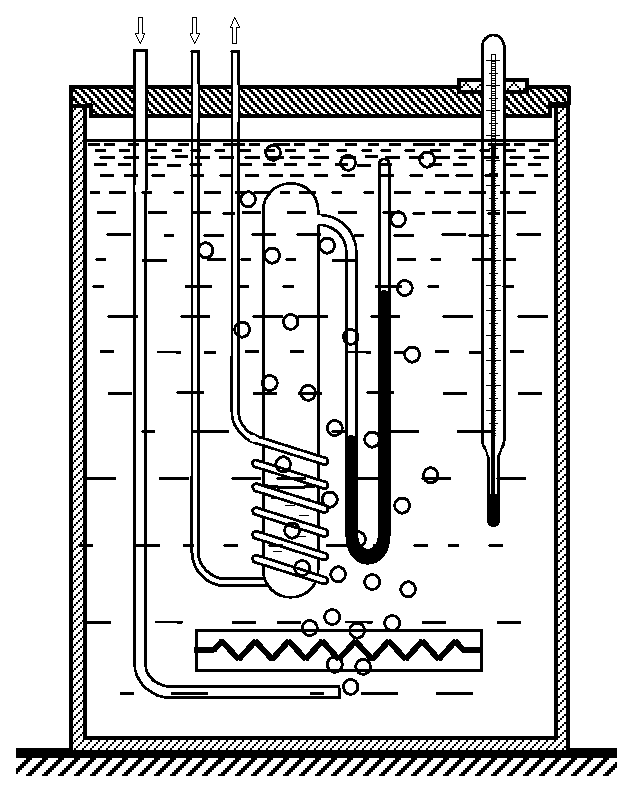
\includegraphics[width=\vva]{pic/O1}}%
%\hfil
%\hbox to \vvb{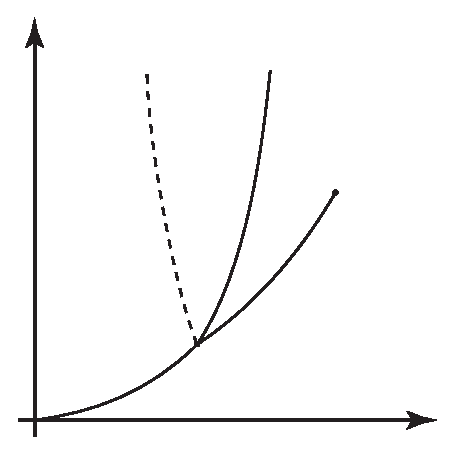
\includegraphics[width=\vvb]{pic/O2}}%

\vfill

\newpage
